\documentclass[a4paper,11pt]{scrartcl} %Standard A4, 11pt Font Größe
\usepackage{fullpage} %weniger Rand
\usepackage[utf8]{inputenc} %richtige Kodierung, auch für Umlaute
% \usepackage{german} %Deutsch mit Zeilenumbrüchen
% \usepackage[german]{babel}
\usepackage{latexsym} %laden von weiteren mathematischen Symbolen
\usepackage{amssymb} % mathematische Symbolzeichensätze (z.B. \mathbb{)
\usepackage{graphicx} %Figures und Subfigures
\usepackage{caption}
\usepackage{subcaption}
\usepackage[obeyspaces,hyphens]{url}
\usepackage{cite}
\usepackage{xcolor}
\usepackage{soul}
\usepackage{amsmath}
\usepackage{algorithm}% http://ctan.org/pkg/algorithms
\usepackage{algpseudocode}% http://ctan.org/pkg/algorithmicx

\definecolor{lightgray}{rgb}{0.6,0.6,0.6}
\definecolor{darkgray}{rgb}{0.3,0.3,0.3}
\newcommand{\err}[1]{$^{\textcolor{red}{#1}}$}
\newcommand{\fl}[1]{\colorbox{lightgray!20}{\path{#1}}}
\newcommand{\cd}[1]{\sethlcolor{darkgray} \textcolor{white}{\hl{\texttt{#1}}}}
\newcommand*{\vv}[1]{\vec{\mkern0mu#1}}

%Header und Titel
\title{N-Body Simulation}
\subtitle{VL Parallele Systeme, HTW Berlin, SS2017}
\author{Richard Remus, Jonas Jaszkowic}
\date{}

%----------------------------------------------------------------------
\begin{document}
\maketitle
% \tableofcontents

\section{Introduction}
Implementing a N-body simulation breaks down to solving the N-body problem of predicting the individual motions of a group of $n$ objects interacting with each other gravitationally. The exact solution to this problem has a time complexity of $\mathcal{O}(n^2)$ which means that it is not possible to solve it efficiently in an appropriate period of time, especially when the number of objects is large. Reducing time complexity can either be done by using approximate methods which produce a "good enough" solution or by parallelizing the algorithm on multi-core processors. For this work, we focus on the latter.

\section{N-body problem}
The N-body problem is a generalized form of the famous two-body and three-body problem which are dealing with the same question: determining the motions of two or three bodies interacting with each other gravitationally. An explicit analytical solution is known to the two-body problem, i.e. simple functions $\vv{r_1}(t)$ and $\vv{r_2}(t)$ that takes only the time $t$ as a parameter and calculates the corresponding position of both bodies given only the initial conditions. However, up to today no analytical solution in the form of $\vv{r_i}(t)$ functions has been found for the three-body problem or the n-body problem. \cite{nbodysolve} The most straight-forward methods are called \textit{direct} methods or \textit{particle-particle} methods. For these problems, a number of numerical solutions are known.
\subsection{Definition}
The n-body problem is given by $n$ point masses $m_i > 0$ and $n$ initial position vectors $\vv{r_i}$ for $i=1,2,...,n$ in a three-dimensional reference system $\mathbb{R}^3$, their mutual gravitational attraction being the single force acting on them. \cite{meyer2008introduction}Given these initial conditions, the task can now be stated as: \textit{Find the position vectors for each body given a time $t$.}
\subsection{Derivation}
Finding the body positions boils down to calculating the acceleration for each body. Using Newton' second law of motion
\begin{align*}
F = m \cdot a 	
\end{align*}\\
we can state that mass times acceleration of the $i$th body is equal to the sum of the forces acting on this particular body. The sum of the forces can be calculated using Newton's universal law of gravity
\begin{align*}
F = \gamma \cdot \frac{m_1m_2}{r^2}	
\end{align*}\\
where $\gamma$ is the gravitational constant, and the superposition principle
\begin{align*}
\vv{F_{res}} = \vv{F_1} + \vv{F_2} + ... + \vv{F_n}	
\end{align*}\\
and the direction of this force defined by
\begin{align*}
\vv{q_j} -\vv{q_i}~/~||\vv{q_j} - \vv{q_i}||
\end{align*}
With these basic laws we can derive the acceleration $a_i$ for every body:
\begin{align*}
	m_i \cdot a_i &= F\\
	m_i \cdot a_i &= \gamma \sum\limits_{j=1}^N \frac{m_i m_j}{||\vv{q_j} - \vv{q_i}||^2}  \\
	\vec{a}^{\,}_i \cdot m_i &= \gamma \sum\limits_{j=1}^N \frac{m_i m_j}{||\vv{q_j} - \vv{q_i}||^2} \cdot \frac{(\vv{q_j} - \vv{q_i})}{||\vv{q_j} - \vv{q_i}||} \\
	\vv{a_i} &= \gamma \sum\limits_{j=1}^N \frac{m_j \cdot (\vv{q_j} - \vv{q_i})}{||\vv{q_j} - \vv{q_i}||^3}
\end{align*}\\
In order to avoid division by zero in the distance calculation $||\vv{q_j} - \vv{q_i}||$ we introduce a softening factor $\epsilon$:

\begin{align*}
	\vv{a_i} &= \gamma \sum\limits_{j=1}^N \frac{m_j \cdot (\vv{q_j} - \vv{q_i})}{(||\vv{q_j} - \vv{q_i}||^2 + \epsilon^2)^\frac{3}{2}}
\end{align*}
With this equation we have deducted the acceleration $\vv{a_i}$ of each body. Using infinitesimal time steps and the laws $v = a\cdot t$ and $s=v\cdot t$, we can iteratively calculate the postion of each body for every time $t$.

\section{Algorithm}
With the above physical equations we can formulate an algorithm for the simulation of the body positions over time given an initial configuration. This algorithm uses the \textit{direct} method and features no further optimizations beside the parallelization that is applied later on. The core algorithm consists of a nested for loop that iterates for each body $i$ over all other bodies $j$ in order to accumulate the forces acting on body $i$. It is important to note that we have to accumulate all forces \textit{before} the calculation of velocity and position can accur, otherwise the update of the position would lead to incorrect results.
\begin{algorithm}[H]
\caption{Update body positions for the given timestep $\Delta$}
\begin{algorithmic}[1]
\Procedure{UpdateStep}{$bodies$,~$\Delta$}
   \For{each body $i$ in $bodies$}
      \State $\vv{a_i} \gets 0$ \Comment{Reset forces for $i$}
      \For{each body $j \neq i$ in $bodies$}
        \State $\vv{a_i} \gets \vv{a_i} + $ CalculateForce($j,i$)
      \EndFor
   \EndFor
   \For{each body $i$}
      \State $\vv{v_i} \gets \vv{v_i} + \Delta * \vv{a_i}$ \Comment{Update velocity}
      \State $\vv{r_i} \gets \vv{r_i} + \Delta * \vv{v_i}$ \Comment{Update position}
   \EndFor
\EndProcedure\\
\Procedure{CalculateForce}{$j,~i$}
	\State \Return $\gamma \frac{m_j \cdot (\vv{q_j} - \vv{q_i})}{(||\vv{q_j} - \vv{q_i}||^2 + \epsilon^2)^\frac{3}{2}}$
\EndProcedure
\end{algorithmic}
\end{algorithm}

Because the calculation of the force for each body is independent of previous steps or partial results the nested for-loop can be fully parallelized. The same applies for the second for-loop that updates the positions and velocities.

\section{Implementation}
The simulation and the core algorithm was implemented in \texttt{C/C++} with OpenMP \cite{openmp} and OpenCL \cite{opencl} as parallelization frameworks. For developing and debugging we used the CLion IDE \cite{clion} on two identical MacBook Pro machines running macOS Sierra.

\subsection{Software design}
TODO: description
\begin{figure}[h!]
	\centering
	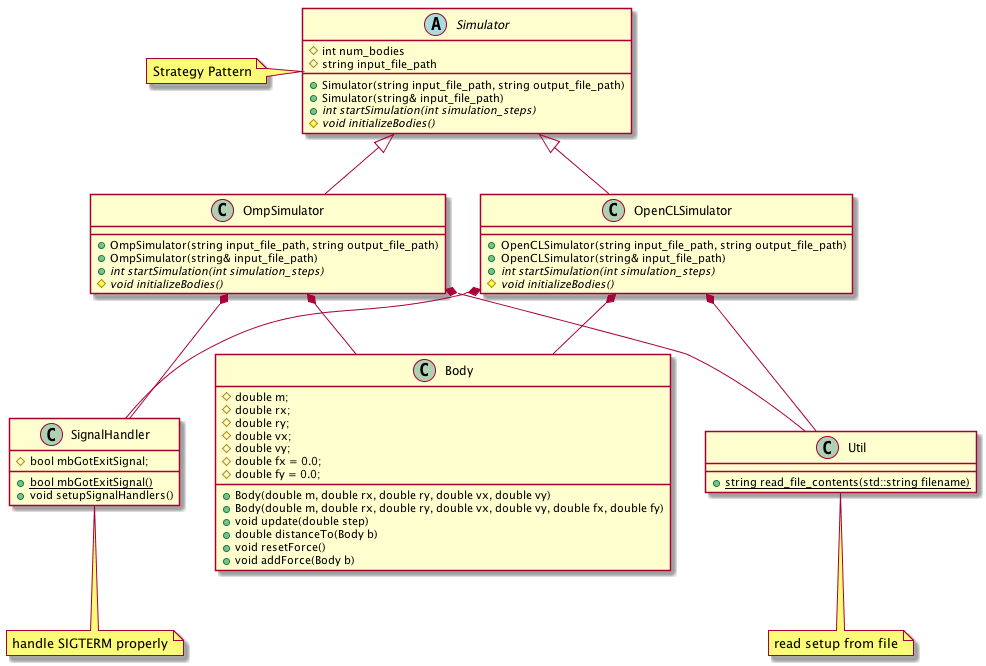
\includegraphics[width=\textwidth]{img/classes.png}
	\caption{Architectural overview of the classes involved in the simulation.}
	\label{fig:classes}
\end{figure}

\subsection{Astronomical Units}
Distances, masses and velocities in the universe lead to large numbers that might not fit in floating
point numbers. Because many OpenCL vendors do not support double precision numbers, we scale these values to astronomical units that will fit in single precision floating points. In astronomical units, time is
measured in years, distances in AU and masses in solar-masses:

\begin{align*}
	1~yr &= 365.25 * 86400~s = 31557600~s \\
	1~AU &= 149597870700~m \\
	1~M &=  1.98892 \cdot 10^{30}~kg
\end{align*}

With these values we can scale the gravitational constant accordingly \cite{astrounits}:

\begin{align*}
	6.674 \cdot 10^{-11} \frac{m^3}{kg \cdot s^2}
	& =  6.674 \cdot 10^{-11} \cdot 2.98692\cdot 10^{-34} \frac{AU^3}{kg \cdot s^2}\\
	& = 6.674 \cdot 10^{-11} \cdot 2.98692\cdot 10^{-34} \cdot 1.98892 \cdot 10^{30} \frac{AU^3}{M \cdot s^2} \\
	& = 6.674 \cdot 10^{-11} \cdot 2.98692\cdot 10^{-34} \cdot 1.98892 \cdot 10^{30} \cdot 9.95844249\cdot 10^{14} \frac{AU^3}{M \cdot yr^2}\\
	& = 39.445 \frac{AU^3}{M \cdot yr^2}
\end{align*}

\section{Parallelization}
\subsection{OpenMP}
TODO: describe used pragmas
\subsection{OpenCL}
TODO: show kernel code, describe concept of work groups

\section{Initital configurations}
TODO: proof of concept with solar system configuration, effect of varying epsilon and gravitational constant, example images

\section{Benchmarks}
TODO: include all benchmarks, test on different machine!


\bibliography{bibliography}{}
\bibliographystyle{plainurl}
\end{document}
